\section{NTK$^{\text{fixed-gate}}\propto$ NPK: Theorem to explain roles of gates, weights, width and depth}

\begin{assumption}\label{assmp:main}
(i) $\Tv_0$ is statistically independent of $\Tf_0$ (ii) $\Tv_0$ are i.i.d symmetric Bernoulli over $\{-{\sigma},+{\sigma}\}$. 
\end{assumption}

\begin{theorem}\label{th:main} Let $\sigma=\frac{\sigfc}{\sqrt{w}}$ in \Cref{assmp:main}. As $w\ra\infty$, for FC-DGN we have: 

\begin{align*}
\kv_{\Tdgn_0}(x,x')&\stackrel{(a)}\ra d \sigma^{2(d-1)} H_{\Tf_0}(x,x')\\ 
%&\stackrel{(a)}{=} d \sigfc^{2(d-1)}\langle x,x'\rangle\cdot \Pi_{l=1}^{d-1} \left(\frac{\langle G_{x,\Tf_0}(l), G_{x',\Tf_0}(l) \rangle}{w}   \right)\\
%&\stackrel{(a)}\propto \langle x,x'\rangle\cdot \Pi_{l=1}^{d-1} \left(\frac{\langle G_{x,\Tf_0}(l), G_{x',\Tf_0}(l) \rangle}{w}   \right)\\
&\stackrel{(b)}= \langle x,x'\rangle\cdot \Pi_{l=1}^{d-1} \frac{H^{\text{lyr}}_{l,\Tf_0}(x,x')}{w}
\end{align*}

\end{theorem}

\FloatBarrier
\begin{figure}[h]
\centering
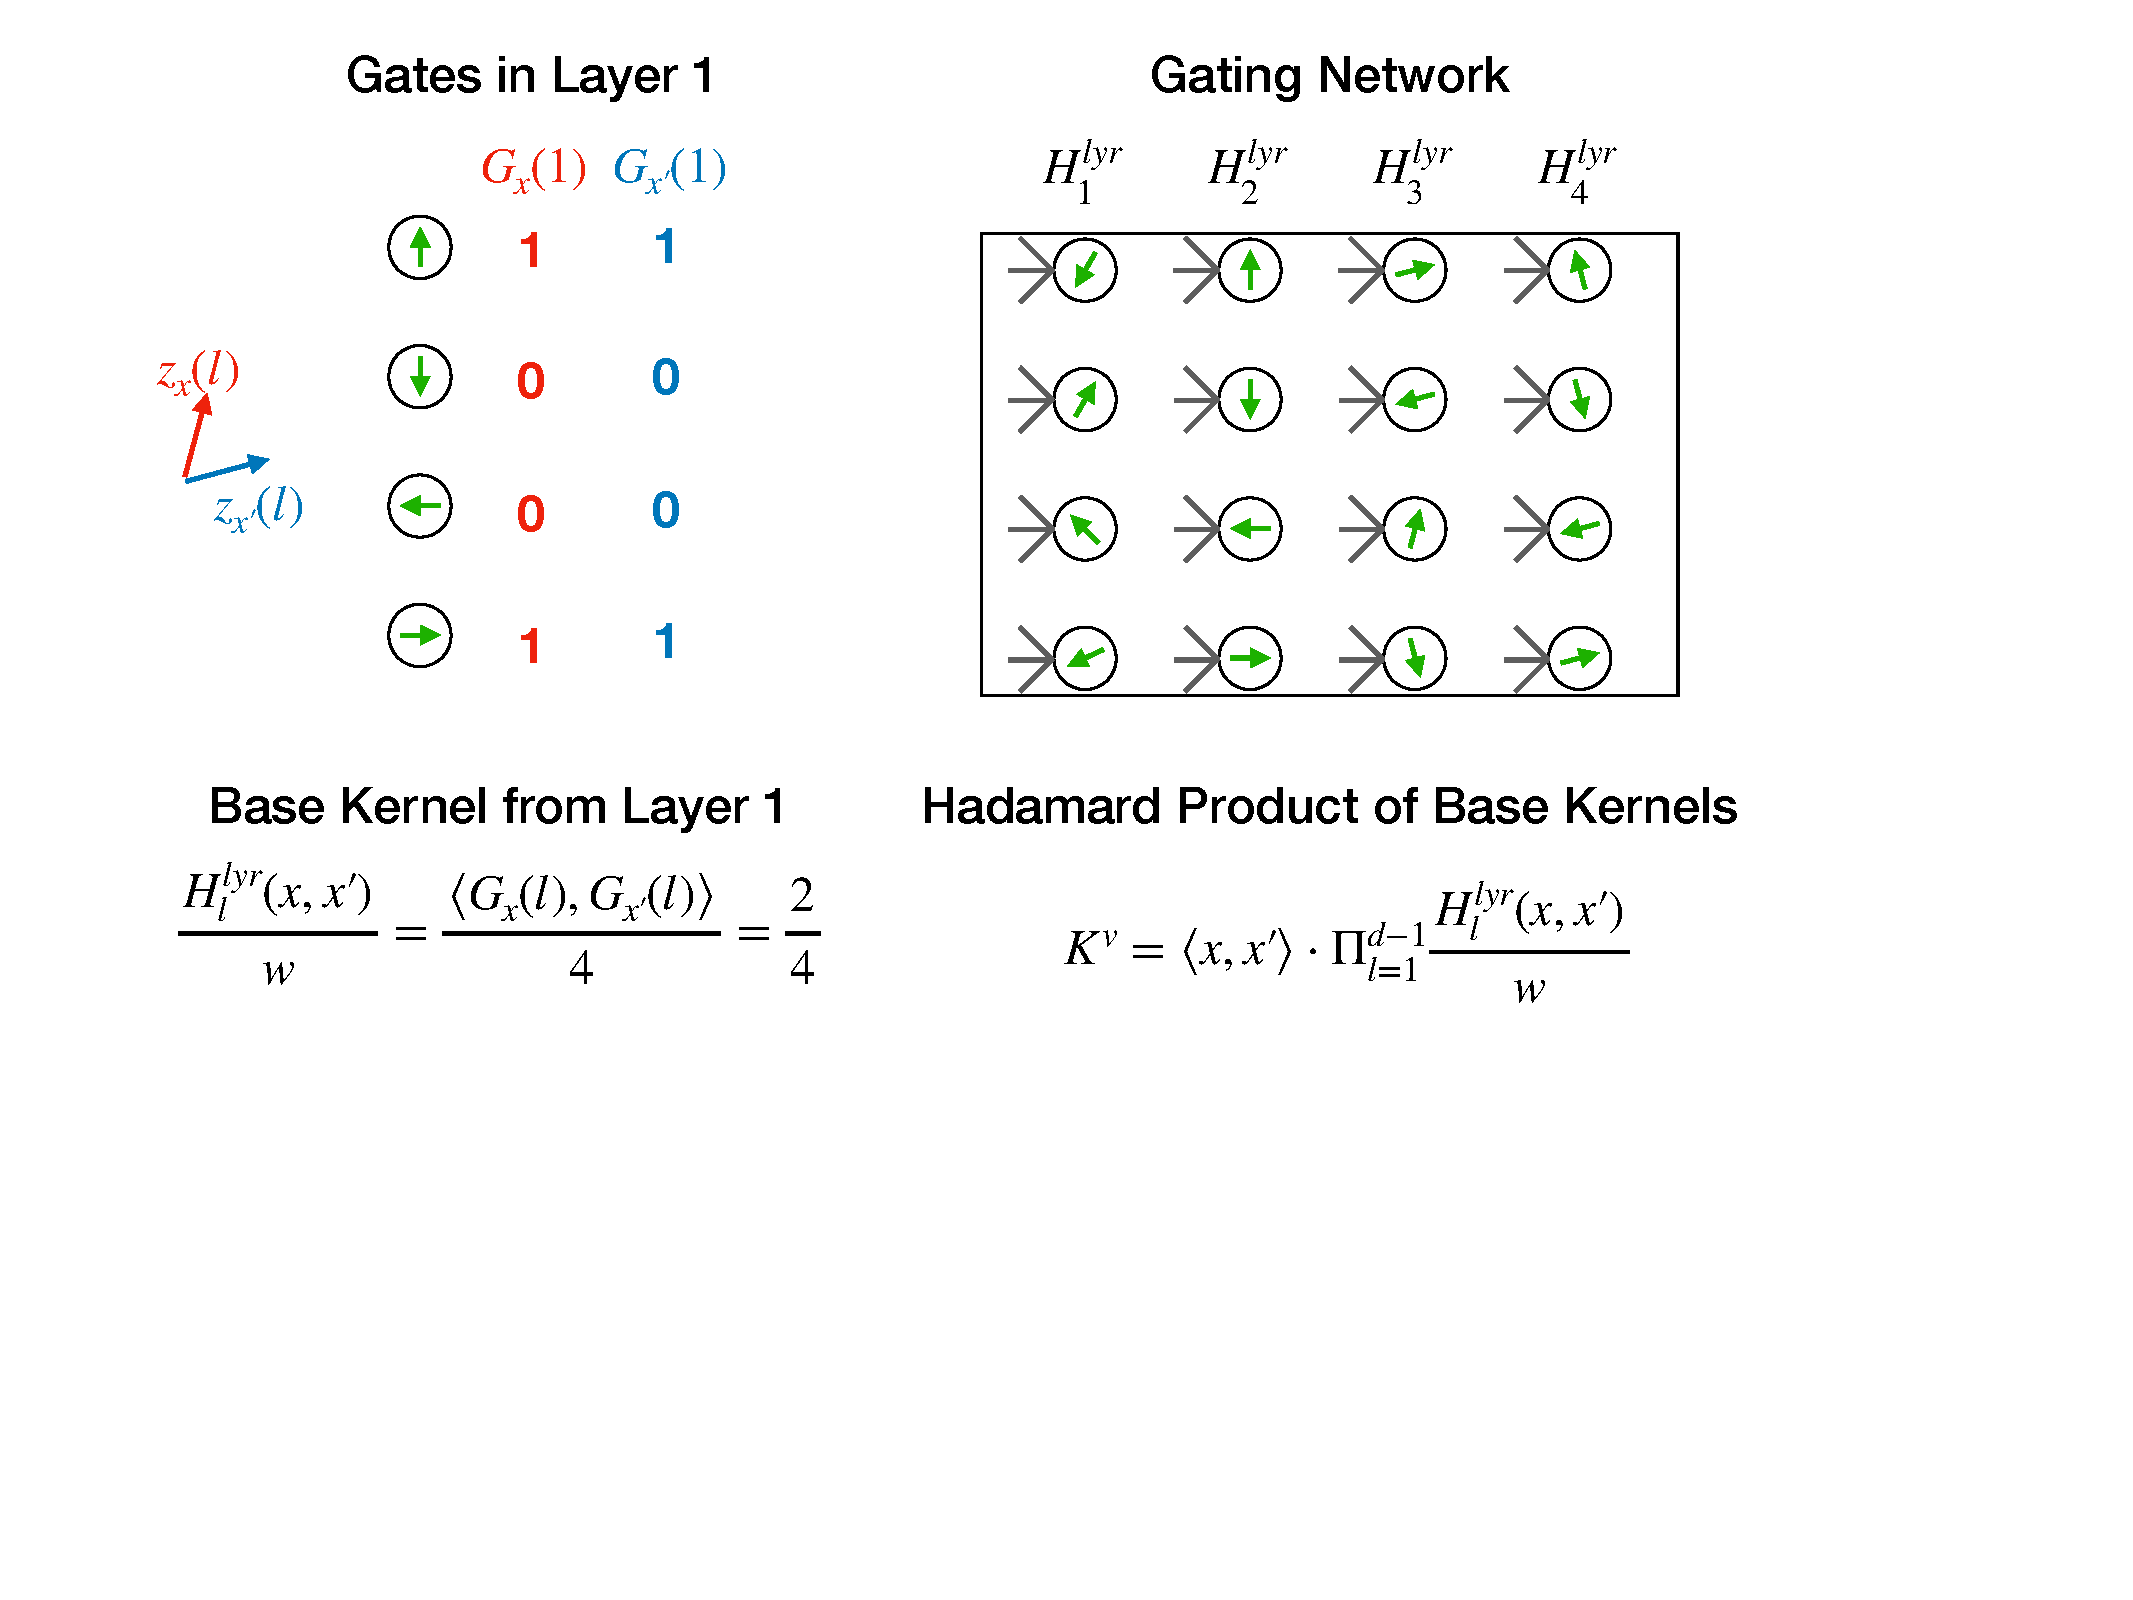
\includegraphics[scale=0.25]{figs/overall.pdf}
\end{figure}